\chapter{Architettura del Sistema Simulato}	
\label{chapter:architettura}

In questo capitolo verranno affrontati innanzitutto i dettagli implementativi del simulatore \textit{YAFS}, la sua struttura e la modellazione delle simulazioni. Successivamente verranno approfondite le caratteristiche degli scenari simulati nel corrente lavoro di Tesi.

\section{Struttura e Funzionamento di YAFS}

Per le simulazioni realizzate nel corrente lavoro di Tesi è stato fatto uso del simulatore \textit{YAFS} \footnote{Disponibile su: \url{https://github.com/acsicuib/YAFS}} (\textit{Yet Another Fog Simulator}) \cite{YAFSSimulator}. Quest'ultimo utilizza una libreria per la generazione e la gestione degli eventi chiamata \textit{SimPy} \footnote{Disponibile su: \url{https://simpy.readthedocs.io}}, ovvero un'implementazione di un simulatore ad eventi discreti (DES, \textit{Discrete Event Simulator}), che garantisce un'interfaccia per la definizione dei processi (i componenti attivi della simulazione) e delle risorse (ad esempio i nodi ed i collegamenti della rete).

YAFS è definito principalmente da sei classi: \textit{Core}, \textit{Topology}, \textit{Selection}, \textit{Placement}, \textit{Population} e \textit{Application}. Le relazioni che intercorrono tra loro sono mostrate in Figura \ref{fig:YAFS_classes} ed esposte nel seguito.

\begin{figure}[!ht]
  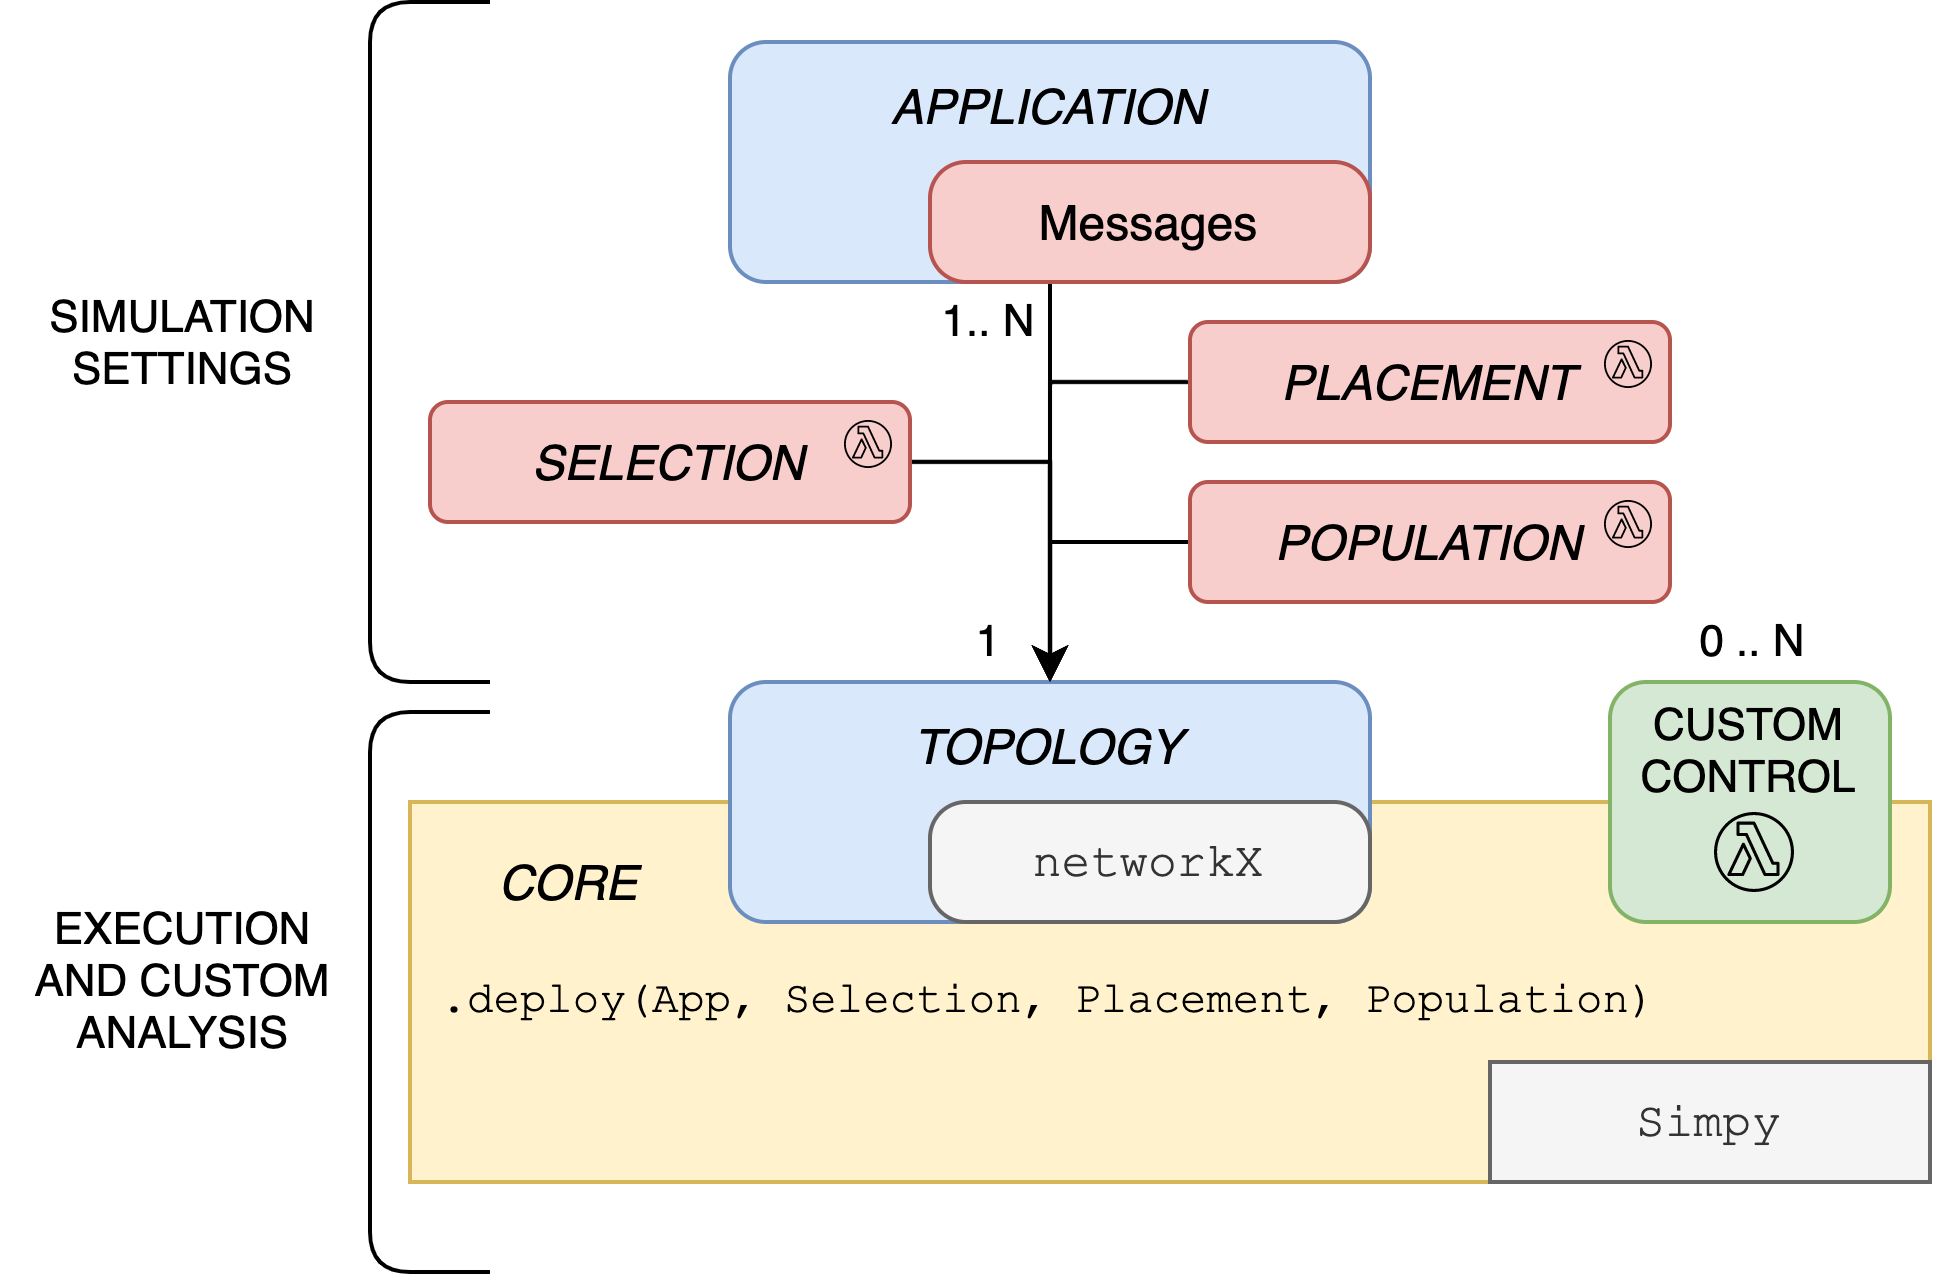
\includegraphics[width=12cm]{images/YAFS_classes}
  \centering
  \caption[Architettura di YAFS]{Architettura di YAFS.\cite{YAFSSimulator}}
  \label{fig:YAFS_classes}
\end{figure}

\subsection{Topologia e Modellazione delle Entità}

Le entità della topologia sono modellate come un insieme di \textit{nodi} (ovvero i dispositivi della rete, come dispositivi IoT, nodi fog, server e cloudlet) interconnessi da \textit{archi} (i collegamenti di rete). La modellazione della topologia, tramite un \textit{grafo} permette l'applicabilità della \textit{Complex Network Theory}. Grazie all'integrazione di \textit{NetworkX}  \cite{NetworkX}, una nota libreria scritta in Python, è possibile applicare algoritmi per eseguire misure e analisi sui grafi, come il calcolo di node degree, centrality, clustering, assortativity, communities e così via. NetworkX accetta inoltre la definizione dei grafi tramite JSON, formato (open e standard) ampiamente utilizzato per la creazione dello scenario con YAFS e permette l'esportazione dei grafi in formato GEXF, utile ad esempio per l'analisi dei grafi tramite il software \textit{Gephi} \footnote{Disponibile su: \url{https://gephi.org/}}.

Gli attributi obbligatori per la definizione di un nodo sono un identificativo univoco (\textit{ID}), il numero di istruzioni eseguite dal nodo in un'unità di tempo (\textit{IPT}) e la capacità della memoria (\textit{RAM}). L'utente è libero di aggiungere attributi personalizzati, utili allo scenario specifico che si vuole studiare, come è stato fatto nel corrente lavoro di Tesi (maggiori informazioni sono al Capitolo \ref{chapter:implementazione}). Un esempio di definizione dei nodi è mostrato nel Listato \ref{lst:node-definition}. 
\begin{lstlisting}[language=json, caption={Definizione di due nodi Fog utilizzando la rappresentazione JSON \cite{YAFSSimulator}}, captionpos=b, label={lst:node-definition}]
{
    "id": 120, "RAM": 1, "IPT": 530,
    "POWERmin": 574,
    "POWERmax": 646,
    "coordinate": 
    {
        "lat": 39.30, "long": 3.34
    }
},
{
    "id": 12, "RAM": 10, "IPT": 100
}
\end{lstlisting}

La definizione dei collegamenti è molto simile. Questi hanno i seguenti attributi obbligatori: la larghezza di banda (\textit{BW}), la velocità di propagazione (\textit{PR}), l'ID del nodo sorgente (\textit{s}) e l'ID del nodo di destinazione (\textit{d}). I valori \textit{BW} e \textit{BR} sono utili al calcolo della latenza secondo la formula:
$$\frac{Message.size.bytes}{BW} + PR$$

\subsection{Modellazione delle Applicazioni}
In YAFS le applicazioni (intese come raggruppamenti di servizi), sono strutturate come dei \textit{Distributed Data Flow} (DDF) \cite{DDF_IOT_App}. In particolare un'applicazione è definita da un insieme di moduli che si scambiano messaggi. Infatti, un DDF è rappresentato da un \textit{grafo diretto aciclico}, dove i nodi sono i moduli che eseguono delle azioni sui messaggi in ingresso, provenienti da un certo percorso sugli archi del grafo. Questa rappresentazione è utile al fine di garantire il partizionamento delle applicazioni e la scalabilità, ad esempio tramite l'implementazione di microservizi \cite{microservices}. 

\begin{figure}[!ht]
  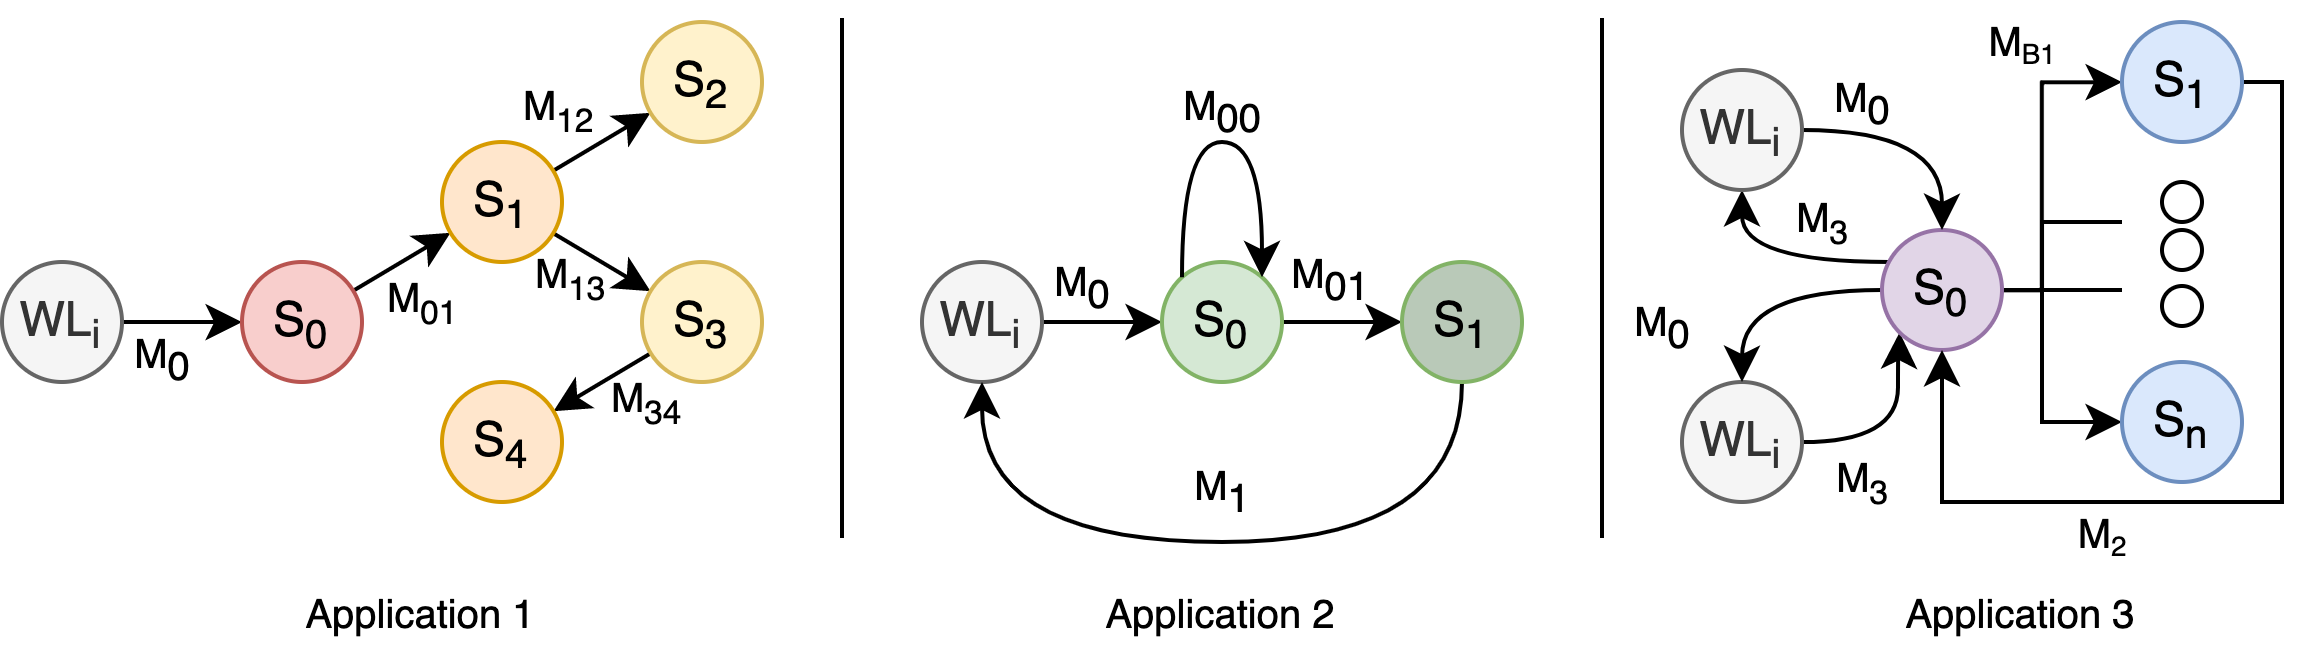
\includegraphics[width=14cm]{images/applications_ddf}
  \centering
  \caption{Tre tipologie di applicazioni realizzabili, con la loro rappresentazione tramite grafo.\cite{YAFSSimulator}}
  \label{fig:applications_ddf}
\end{figure}

La definizione delle applicazioni è composta da quattro parti: \textit{moduli} (o \textit{servizi}), \textit{messaggi}, \textit{trasmissioni} e dati generali. I \textit{moduli} possono avere diversi attributi, anche a seconda dello specifico scenario, ma quelli obbligatori sono solo un identificativo univoco (\textit{ID}) e il nome (\textit{name}). I \textit{messaggi}, ovvero i dati scambiati, hanno principalmente due attributi obbligatori: il numero di istruzioni (\textit{instructions}) e la grandezza in byte (\textit{bytes}). Le \textit{trasmissioni} definiscono le modalità in cui i servizi scambiano le informazioni e tramite le quali si inviano dati. Gli attributi obbligatori in questo caso sono: il modulo di afferenza (\textit{module}) e il messaggio in ingresso. Tramite la definizione delle trasmissioni è possibile, con un particolare attributo detto \textit{fractional}, definire la probabilità di propagare un determinato messaggio \textit{message\_out} sulla ricezione di un particolare messaggio \textit{message\_in}. 

In Figura \ref{fig:applications_ddf} sono mostrate tre tipologie di applicazioni che sono realizzabili. La prima, \texttt{Application 1}, è strutturata gerarchicamente, con la ricezione dei messaggi $M_{ij}$ che scatena l'invio di altri messaggi. Nella seconda applicazione, \texttt{Application 2}, è possibile osservare un'interazione di un servizio con se stesso ed infine nell'ultima applicazione, \texttt{Application 3}, è mostrato il \textit{broadcasting} di un messaggio $M_{B1}$ che raggiunge tutti i moduli dell'applicazione. In tutte e tre le applicazioni $WL_i$ indica il nodo che genera il carico di lavoro (ad esempio un dispositivo IoT).

\subsection{Politiche dinamiche}
Le classi \textit{Selection}, \textit{Placement} e \textit{Population} sono utili per la generazione dinamica degli eventi dello scenario. In particolare la prima definisce quali nodi devono eseguire un particolare servizio, di conseguenza indirizza il \textit{workload}. La classe \textit{Placement} sceglie i servizi che devono essere allocati nei vari nodi, mentre la class \textit{Population} posiziona i generatori del workload nei nodi della rete. Queste tre classi possiedono principalmente due interfacce: una contenente l'\textit{initialization function}, che prepara l'allocazione dei moduli e del workload nei nodi della rete, e una contenente una funzione che viene invocata secondo una specifica distribuzione temporale.

\begin{lstlisting}[language=python, caption={Definizione di due Population policies: una statica (\texttt{popA}) ed una dinamica (\texttt{popB}) \cite{YAFSSimulator}}, captionpos=b, label={lst:population-policy}]
delayActivation = deterministicDistributionStartPoint(300, 300, name='Deterministic')
periodActivation = deterministicDistribution(name='Deterministic', time=100)

popA = Statical(name='StaticalPop')
popA.set_sink_control({'id': a_id_fog_device, 'number': 2, 'module': appA.get_sink_modules()})
popA.set_src_control({'number': 1, 'message': appA.get_message('M.Action'), 'distribution': periodicActivation})

top20Devices = [''array_ids_fog_devices'']
popB = Evolution(top20Devices, name='DynamicPop', activation_dist = delayActivation)
popB.set_sink_control({'model': 'actuator-device', 'number': 2, 'module': appB.get_sink_control()})
popB.set_src_control({'number': 1, 'message': appB.get_message('M.action'), 'distribution': periodicActivation})

\end{lstlisting}

Nel Listato \ref{lst:population-policy} è mostrato un esempio di definizione di politiche di \textit{Population}: una statica ed una dinamica. Nelle righe 1 e 2 vengono definite due distribuzioni temporali: la prima che inizia a 3000 unità temporali e da quel punto in poi invoca un'attivazione ogni 300 unità temporali, la seconda invece che invoca un'attivazione ogni 10 unità temporali. Alla riga 4 viene generata un'istanza di una classe Population predefinita. Le applicazioni YAFS hanno due tipi di moduli: \textit{workload sources} e \textit{workload sinks} (interpretabili come ``sensori" ed ``attuatori"). Le righe 5 e 6, tramite JSON, definiscono l'allocazione dei moduli sink e dei moduli source con una specifica distribuzione e il tipo di messaggio che questi devono trattare.

Nel caso della seconda politica di \textit{Population}, viene utilizzato un modello più complesso (righe 8-11): alla riga 9 viene istanziato un oggetto Evolution (Listato \ref{lst:population-evolution}). Questo segue la distribuzione di riga 1, dunque, il processo DES creato, inizia a produrre messaggi dopo un certo intervallo di tempo secondo una specifica scadenza. Ad ogni attivazione il processo creato genera workload con le caratteristiche definite alla riga 11.

\begin{lstlisting}[language=python, caption={Struttura di una classe Population \cite{YAFSSimulator}}, captionpos=b, label={lst:population-evolution}]

class Evolution(population):
	def __init__(self, listIDEntities, **kwargs):
		# initialization of internal variables
		super(Evolutionm self).__init__(**kwargs)
	
	def initial_allocation(self, sim, app_name):
		# dealing assignments
		sim.deploy_sink(app_name, node=fog_device, module=module)
	
	def run(self, sim):
		# dealing assignements: msg, distribution and app_name
		id = ... # listIDEntities.next
		idsrc = sim.deploy_source(app_name, id_node=id, msg=..., distribution=...)

\end{lstlisting}

Nel Listato \ref{lst:population-evolution} è mostrata una versione semplificata della classe Evolution. In questo tipo di classi è sempre presente una funzione obbligatoria chiamata \texttt{initial\_allocation} e, facoltativamente, una funzione chiamata \texttt{run} che viene chiamata secondo l'eventuale distribuzione temporale specificata.

\section{Descrizione dello scenario simulato}

L'architettura di riferimento per la definizione dello scenario simulato è illustrata in Figura \ref{fig:architettura_scenario}.

\begin{figure}[!ht]
  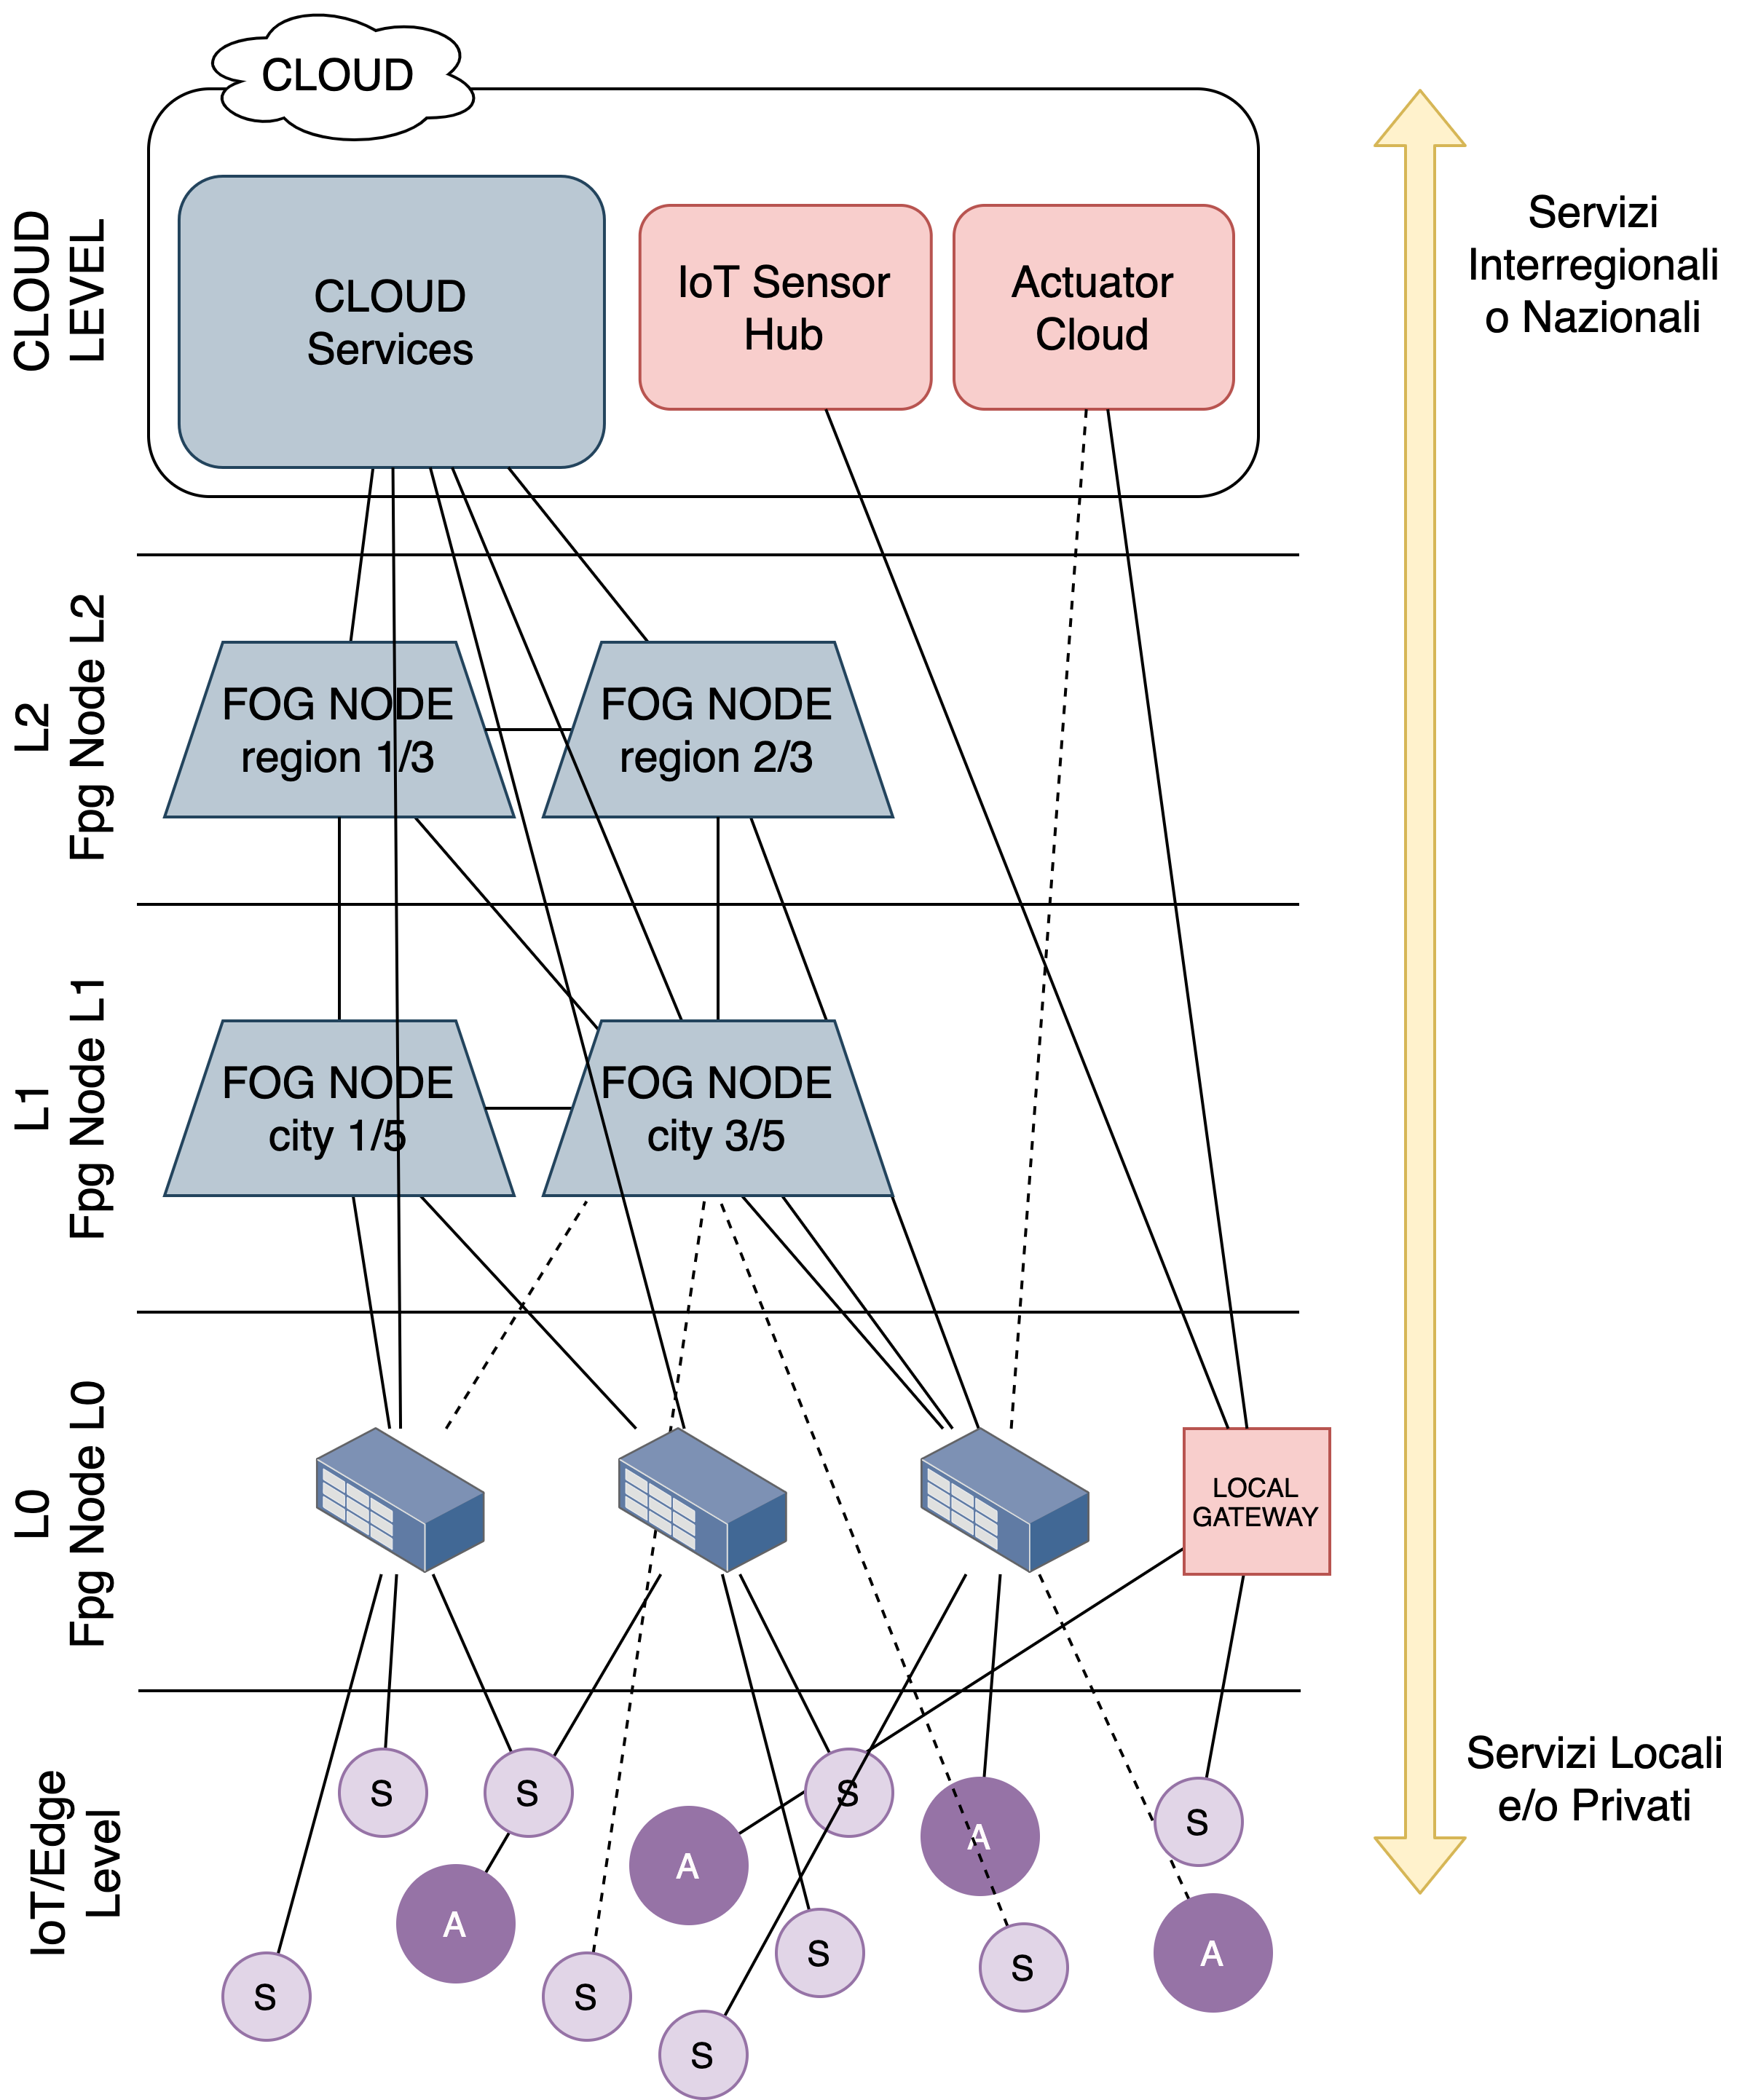
\includegraphics[width=14cm]{images/architettura_scenario}
  \centering
  \caption{Architettura dello scenario simulato}
  \label{fig:architettura_scenario}
\end{figure}

Tra i vari aspetti considerati durante la definizione della topologia di rete si è voluto enfatizzare il concetto del Fog Computing come ``architettura verticale". Dall'esempio in Figura \ref{fig:architettura_scenario} è infatti possibile evincere una struttura della rete gerarchica ed a livelli. Ogni livello è caratterizzato da diverse capacità di elaborazione, in base ai servizi offerti alla rete: un nodo a livelli più bassi offre pochi servizi, ma generalmente produce molti dati (si pensi ad esempio ai dispositivi IoT), mentre un nodo a livelli più alti non genera dati \textit{propri}, piuttosto offre una rielaborazione dei dati ricevuti dai livelli più bassi offrendo molti servizi alla rete.

Un fattore di particolare rilevanza è inoltre la \textit{raggiungibilità}. Ricordando infatti la necessità di rendere i servizi della rete disponibili anche nelle zone più remote della stessa, ovvero vicino all'\textit{edge} per ridurre al minimo la latenza, i nodi appartenenti a livelli più bassi sono più radicati nel territorio ed ognuno di essi è raggiungibile da aree via via più limitate e circoscritte. 

\subsection{Architettura a livelli}

Il sistema simulato in questo lavoro di Tesi offre degli spunti per l'implementazione del Fog Computing in scenari anche molto differenti tra loro. Infatti viene proposta una architettura a livelli molto flessibile e adattabile a diversi tipi di implementazioni, che possono avere qualsiasi estensione geografica a seconda delle diverse esigenze.

\subsubsection{Livello IoT/Edge}

In questo livello vengono raggruppati i sensori e gli attuatori che rientrano nell'ambito IoT, cioè dispositivi caratterizzati da una bassa capacità computazionale, scarsa alimentazione, discontinuità e mobilità. I dispositivi che operano in questo livello utilizzano protocolli di comunicazione a basso consumo, con un \textit{payload} ridotto e tempi di \textit{sleep} prolungati. La caratteristica fondamentale di questi dispositivi è infatti che, per ridurre i consumi, rimangono per tempi molto prolungati in una fase di \textit{sleep}, nella quale il dispositivo resta senza alimentazione (tranne per la circuiteria fondamentale), per poi passare allo stato di \textit{awake}, nel quale vengono eventualmente inviati o ricevuti i dati, tornando immediatamente nello stato di \textit{sleep}.

In 	questo livello vengono inclusi anche i cosiddetti nodi \textit{edge}, il cui scopo è quello di eseguire validazione o controllo dei dati inviati o ricevuti. In particolare questi dispositivi sono generalmente centraline per attuatori o stazioni per sensori più performanti che possono controllarne un numero più consistente.

\subsubsection{Livello Fog $L0$}

In questo livello sono raggruppati i nodi che forniscono i servizi che non rientrano strettamente nell'ambito IoT, ma che non ne offrono ai livelli superiori. Sono ad esempio i cosiddetti \textit{gateway}, spesso privati, che raggruppano sensori e attuatori di zone circoscritte per il loro monitoraggio.

\subsubsection{Livello Fog $L1$}

In questo livello si trovano i nodi che si occupano di raccogliere ed aggregare i dati provenienti da più zone o che offrono semplicemente alcuni servizi alla rete. Questi nodi possono avere, ad esempio, una copertura provinciale o sub-provinciale. Questi offrono diversi servizi alla rete, sia ai i livelli superiori che ai quelli inferiori, ad esempio fornendo raccolta dati per il mantenimento dello storico per i livelli inferiori e fornendo pre-elaborazione degli stessi per i livelli superiori. Le capacità di questi nodi sono piuttosto limitate, ma hanno il grande vantaggio di essere replicabili al fine di garantire la scalabilità. Nel caso di sovraccarico è inoltre possibile sfruttare ad esempio l'operazione di \textit{offloading}\footnote{Con \textit{offloading} si intende il trasferimento di attività computazionali ad alta intensità ad un processore separato, come un acceleratore hardware o ad una piattaforma esterna, come un cluster o il cloud. L'\textit{offload} dell'elaborazione su un nodo esterno può fornire maggiore potenza di elaborazione e superare i limiti hardware di un dispositivo, come potenza di calcolo, archiviazione ed energia limitate.} su nodi vicini dello stesso livello.

\subsubsection{Livello Fog $L2$}
I nodi presenti in questo livello (e negli eventuali successivi Livelli Fog $LN$) hanno una copertura maggiore rispetto a quella dei livelli precedenti, ad esempio regionale o sub-regionale. Come anticipato in questo modello architetturale, i nodi ai livelli superiori hanno capacità computazionali via via sempre maggiori e sono quindi in grado, ad esempio,  di aggregare maggiormente i dati, effettuare veloci analisi statistiche o implementare algoritmi di Machine Learning.

\subsubsection{Livello Cloud}

In questo livello vengono raggruppati i servizi controllati dai produttori dei sensori e degli attuatori (si pensi ad esempio ai servizi utili a raccogliere dati rilevati o ad inviare particolari segnali di controllo agli attuatori), nonché i servizi che richiedono risorse elevate per eseguire, ad esempio, algoritmi di Machine Learning o analisi statistiche avanzate. Nel Capitolo \ref{chapter:implementazione} verrà inoltre spiegato come il Cloud sia un tassello fondamentale per l'algoritmo di Placement, fungendo da ``riserva" per i servizi che non trovano un nodo utile per il piazzamento.

\subsection{Interconnessioni tra Livelli e Scambio di Messaggi}
\label{section:interconnesione_livelli}
Una delle caratteristiche del Fog Computing è la flessibilità della sua implementazione. Infatti i nodi, seppur ordinati gerarchicamente, non sono necessariamente connessi con i nodi ai livelli subito successivi o precedenti, ma possono essere eventualmente connessi con qualsiasi altro livello superiore o inferiore. 

Per quanto riguarda invece le interconnessioni interne ai livelli, queste seguono diverse modalità. Nel caso dei livelli IoT/Edge e Fog $L0$ generalmente non sono previste connessioni, mentre nei livelli Fog da $L1$ ad $LN$ viene utilizzato un grafo \textit{small-world}\footnote{Una rete \textit{small-world}, è un tipo di grafo in cui la maggior parte dei nodi sono uno vicino (\textit{neightbors}) dell'altro e dato un nodo, i suoi vicini sono molto probabilmente vicini tra loro, con il risultato che ogni nodo è raggiungibile dall'altro con un ridotto numero di \textit{hop}.} secondo il modello \textit{Watts-Strogatz} \cite{WattsStrogatzModel}.

Il sistema simulato è un'implementazione di un'architettura basata sullo scambio di messaggi tra i servizi. Questo avviene tramite un'operazione di \textit{replay} dei messaggi che avviene secondo specifiche distribuzioni di probabilità, che diminuisce ai livelli superiori. Ad esempio un messaggio generato dal Livello IoT/Edge raggiunge il livello $L0$ con probabilità pari a $0.8$, il livello $L1$ con probabilità pari a $0.4$ e così via.



















